% small.tex

\documentclass{beamer}


\usetheme{default}

\title{ECE411 Final Presentation}
\subtitle{Womprats T-16 Audio Synthesizer}
\author{A. Goetz \and B. Kanyid \and J. Pugh \and K. Riedl}
\institute[PSU]{
  Maseeh College of Engineering and Computer Science\\
  Portland State University\\
  Portland, Oregon 97207  
}
\date{\today}

\begin{document}

\begin{frame}[plain]
  \titlepage
\end{frame}


\begin{frame}{Problem}

  \textbf{Problem Statement:}  \pause Build something cool in order to
  practice for engineering capstone. 

  \pause \textit{Okay, what really is the goal of this project?}

  \pause Use both hard engineering and soft people skills to
  successfully develop a product in a ten week period. 
  
  \pause \textit{Yeah, but what did you actually build?}

  \pause Design and implement a multi-channel audio-synthesizer for
  chiptune music.

  
\end{frame}

\begin{frame}{Motivation}
%% Why is it important? What is the value of a solution (lives, money,
%% effort, energy saved)?

  Our solution provides a simple interface that allows the generation
  of complex waveforms. 

  On a higher level, it demonstrates that we can balance real-world
  engineering tradeoffs in a practical project. 

\end{frame}

\begin{frame}{Objective}

  Our objective is to design, build and test an audio synthesizer
  capable of mixing multiple waveforms to create a single audio out. 
\end{frame}

\begin{frame}{Alternatives}
%% How is it done today or what other alternatives exist?

There are many synthesizer products on the market today. Our goal is
not to compete with these products, but to create something that is realizable in 10 weeks. 
\end{frame}

\begin{frame}{Requirements}
%% What are the requirements for an acceptable solution?  

\end{frame}

\begin{frame}{Our Approach}
Brief overview of your approach
\end{frame}

\begin{frame}{Design}
May need multiple sub-headings here (e.g.  H/W and S/W, or multiple
subsystems) Describe design using appropriate methods (e.g.  UML
models, algorithms) Discuss design alternatives, trade-offs, decisions
made
\end{frame}

\begin{frame}{Implementation}
Details of implementation (major components, schematics, board layout,
code)	  
Tools employed (e.g.  simulation/modeling tool, PCB layout, IDE,
cross-compilers)
\end{frame}

\begin{frame}{IP and Prior Work}
Brief summarize what use you made of prior work or IP including but
not limited to ideas, designs, schematics, board layouts, code.
\end{frame}

\begin{frame}{Testing}
What was the testing strategy and plan?  
\end{frame}

\begin{frame}{Results}
What worked? How well? What didn't? Why?
  
\end{frame}

\begin{frame}{Contributions}
What were the contributions of each member (e.g.  who did PCB, coding,
testing, writing)?
  
\end{frame}
\begin{frame}{Lessons}
What did each member of the team learn as a result of the project
(technical, skill, personal)?  What would you do differently?
\end{frame}

\begin{frame}{PCB}
\begin{center}
 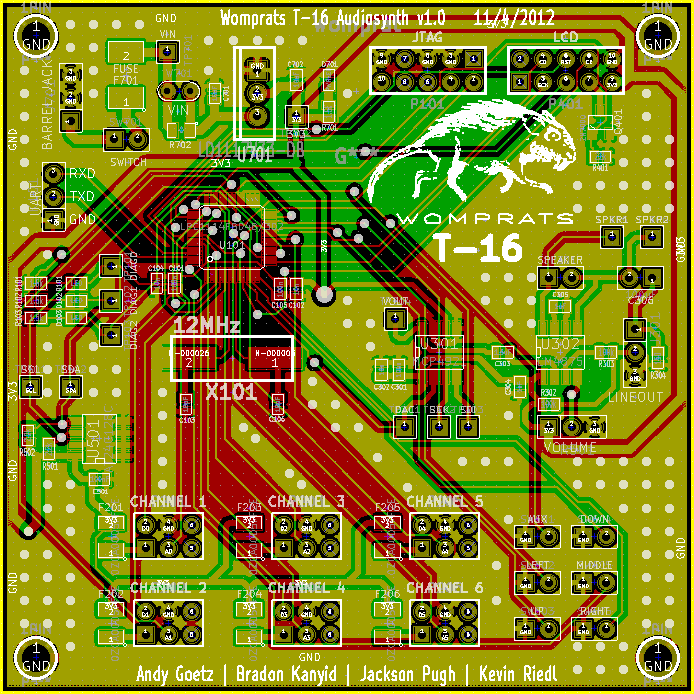
\includegraphics[width=0.7\textwidth]{pcb.png}
\end{center}
\end{frame}

\begin{frame}{Lessons Learned}
  \begin{itemize}
    \pause
  \item KiCad
    \pause
  \item LPC1114
    \pause
  \item GanttProject
    \pause
  \item \LaTeX
    \end{itemize}
\end{frame}


\end{document}
